%
% latex template for SAS documentation 
% name: sas.tex 
% date last modified: 18 mar 2018
% modified by: guru
% 
%
\documentclass{article}

	\usepackage{caption}
	\usepackage[margin=1in]{geometry}
	\usepackage{graphicx}
	\usepackage{hyperref}
	\usepackage{float}
	\usepackage{tabularx}
	\usepackage{titling}
	
	\begin{document}
	
	\title{
		
\includegraphics{images/um_logo.png} \\
		\vspace{0.1in}
		CSC431 \\
		\vspace{0.2in}
		\textbf{Download of Public-facing Data} \\
		\large System Architecture Specification \\
		Team \#3
	}
	
	\author{
		Jerry Bonnell
		\and Gururaj Shriram
		\and Re Chang
		\and Heyu Yao
		\and Lixiong Liang
	}
	
	\date{}
	\maketitle
	
	\clearpage
	\section*{Version History}
	
	\begin{tabularx}{\textwidth}{| l | l | X | l |}
		\hline
		\textbf{Version} & \textbf{Date} & \textbf{Author(s)} & \textbf{Change Comments} \\
		\hline
		1 & \today & Jerry Bonnell and Gururaj Shriram & First Draft \\
		\hline
	\end{tabularx}
	
	\clearpage
	\tableofcontents
	
	\clearpage
	\listoffigures
	\listoftables
	
	\clearpage
	
	\section{System Analysis}
	
	\subsection{System Overview}
	
	The System will be comprised of four main parts: a data manager, data packager, data converter, and REST controller. The data manager will control the connection to the database and handle database queries. The data packager will package all requested pieces of data into a compressed file if multiple pieces of data are requested. The data converter will convert data from the database into the user's desired format. This format can be any of the supported file formats: kml, esri Shapefile, or geoJSON. The REST controller will manage all of the other aspects of the system and manage the end-to-end pipeline of the downloading process. \\
	
	This pipeline is as follows: (1) the browser submits a download request to the download server which the REST controller listens to, (2) the controller initiates the process of querying data from the database based on the list of layers provided by the browser request, (3) the data is then converted to the requested output format, and (4) the server packages data before submitting it to the browser for local download. \\ 
	
	The three-tier architecture will be used for this project. The client-server tier allows the download server to handle requests from the search team. The database-centric tier queries the database to obtain geospatial data. The business layer performs the conversion and archival of this data, before the client-server tier sends the packaged data back to client.   
	
	\subsection{System Diagram}

	\begin{figure}[H]
		\begin{center}
			\caption{Download System Diagram}
			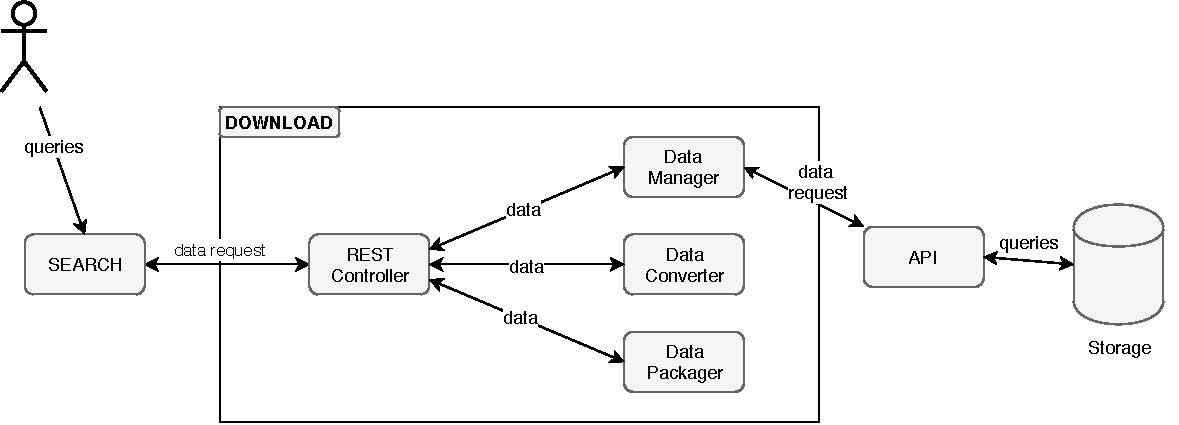
\includegraphics[width=\textwidth]{images/component.pdf}
		\end{center}
	\end{figure}
	
	\clearpage
	
	\subsection{Actor Identification}
	
	There are three types of human actors: unauthorized users, authorized users, and the administrators. Unauthorized users may only download public pieces of data unless they are granted permission to specific pieces of data from an administrator. Authorized users are allowed to download any piece of data. Administrators are able to download any piece of data as well as approve requests for unauthorized users to download private pieces of data. There are currently no plans for the system to support non-human actors, i.e. with an API. 
	
	\subsection{Design Rationale}
	
	\subsubsection{Architectural Style}
	
	This system, which is part of a larger system, solely exists on the back-end. In designing this, we are using the 3-tier architectural style because our system is a back-end API. This lends itself to a natural division into three tiers: client-server, business, and database-centric. In the client-server tier, the REST controller receives user input, validates the input, and passes that on to be processed by the business tier before responding to the client's request. The business tier requests data from the database-centric tier, converts that data and, finally, archives the converted data and sends it back to the client-server tier. The sole purpose of the database-centric tier is to interface with the database. 
	
	\subsubsection{Design Pattern(s)}
	
	Express is a flexible Node.js framework that provides a robust set of features. We predict that the following design patterns will be primarily used in the following ways: \\
	
	\begin{itemize} 
		\item Factory: To abstract objects that may share common tasks, such as data management and parsing objects
		\item Singleton: To maintain a single, consistent reference, such as a database reference
		\item Middleware: To handle flows that have middleware functions in the system's request-response cycle, such as in the data conversion process
		\item Stream: To process large amounts of flowing data, such as in the file writing/core download process
	\end{itemize}
	
	
	\subsubsection{Framework}
	
	The web application will run on the \texttt{Node.js} JavaScript engine on the \texttt{Express} framework. \texttt{Express} allows for the successful implementation of a REST API on the backend and will facilitate a lightweight, efficient download pipeline. \\
	
	\textbf{Links:}
	\begin{itemize} 
		\item \url{https://nodejs.org}
		\item \url{https://expressjs.com}
	\end{itemize}
	
	\clearpage
	
	\subsection{Cross-cutting Requirements}
	
	We have identified two cross-cutting requirements that are involved in performing a download: 
	
	\begin{enumerate}
	\item Performing a \textbf{download}.
	
	Performing a download requires the implementation of a download button on the UI, which calls our download web server, and, at some point, makes contact with the storage database. Therefore, this is a cross-cutting requirement involving three teams that are heavily dependent on each other: search/UI, download, and database. \\
	
	\item Gathering \textbf{geospatial data} from a database.
	
	Further, from the list of layers, our server must be able to gather geospatial data from the Postgres database. This is cross-cutting between the database and our download team.
	
	\end{enumerate}
	
	\clearpage
	
	\section{Functional Design}
	
	% use case should not be included here. 

	\begin{figure}[H]
		\begin{center}
			\caption{Download Sequence Diagram}
			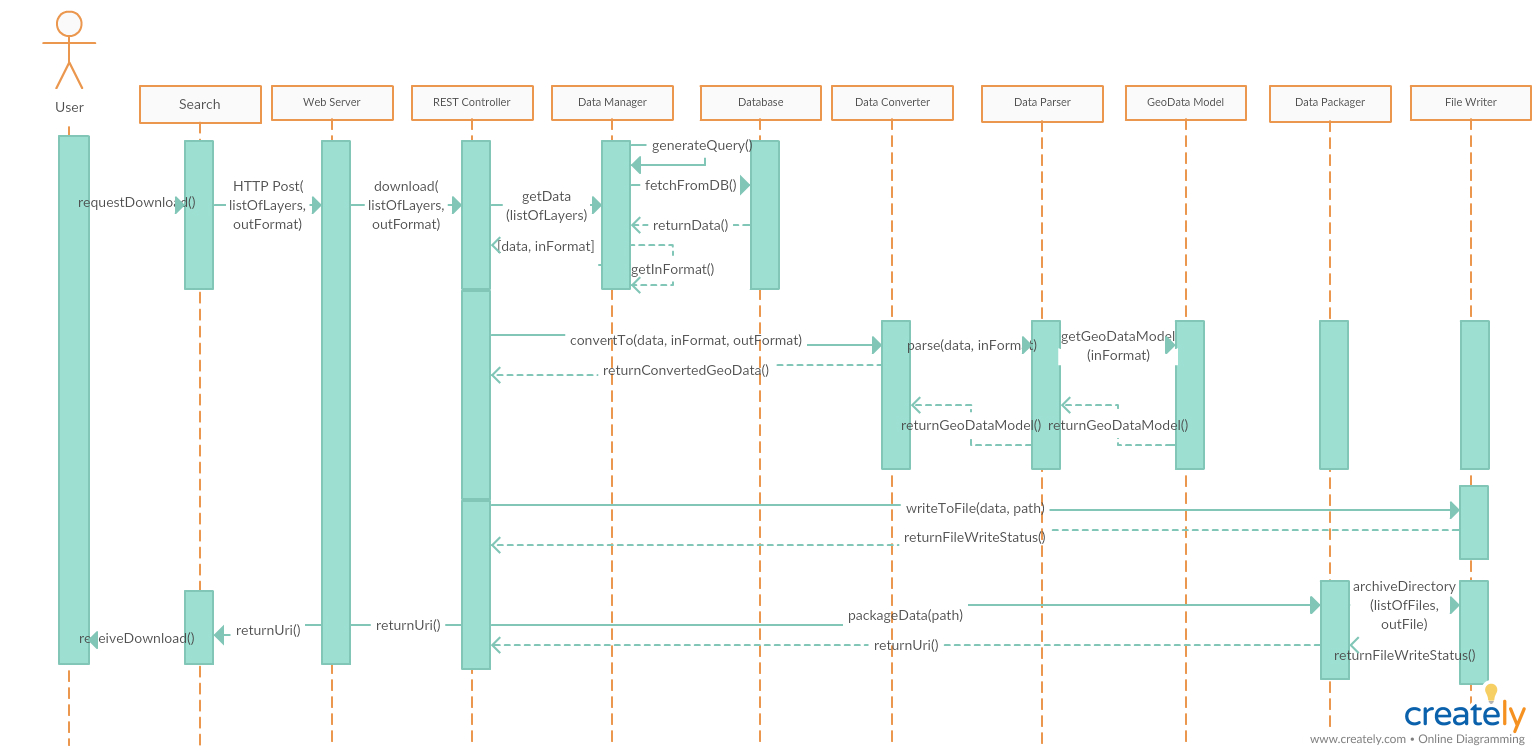
\includegraphics[width=\textwidth]{images/download_sequence_diagram.jpg}
		\end{center}
	\end{figure}

	\clearpage
	
	\section{Structural Design}
	
	\begin{figure}[H]
		\begin{center}
			\caption{Download Class Diagram}
			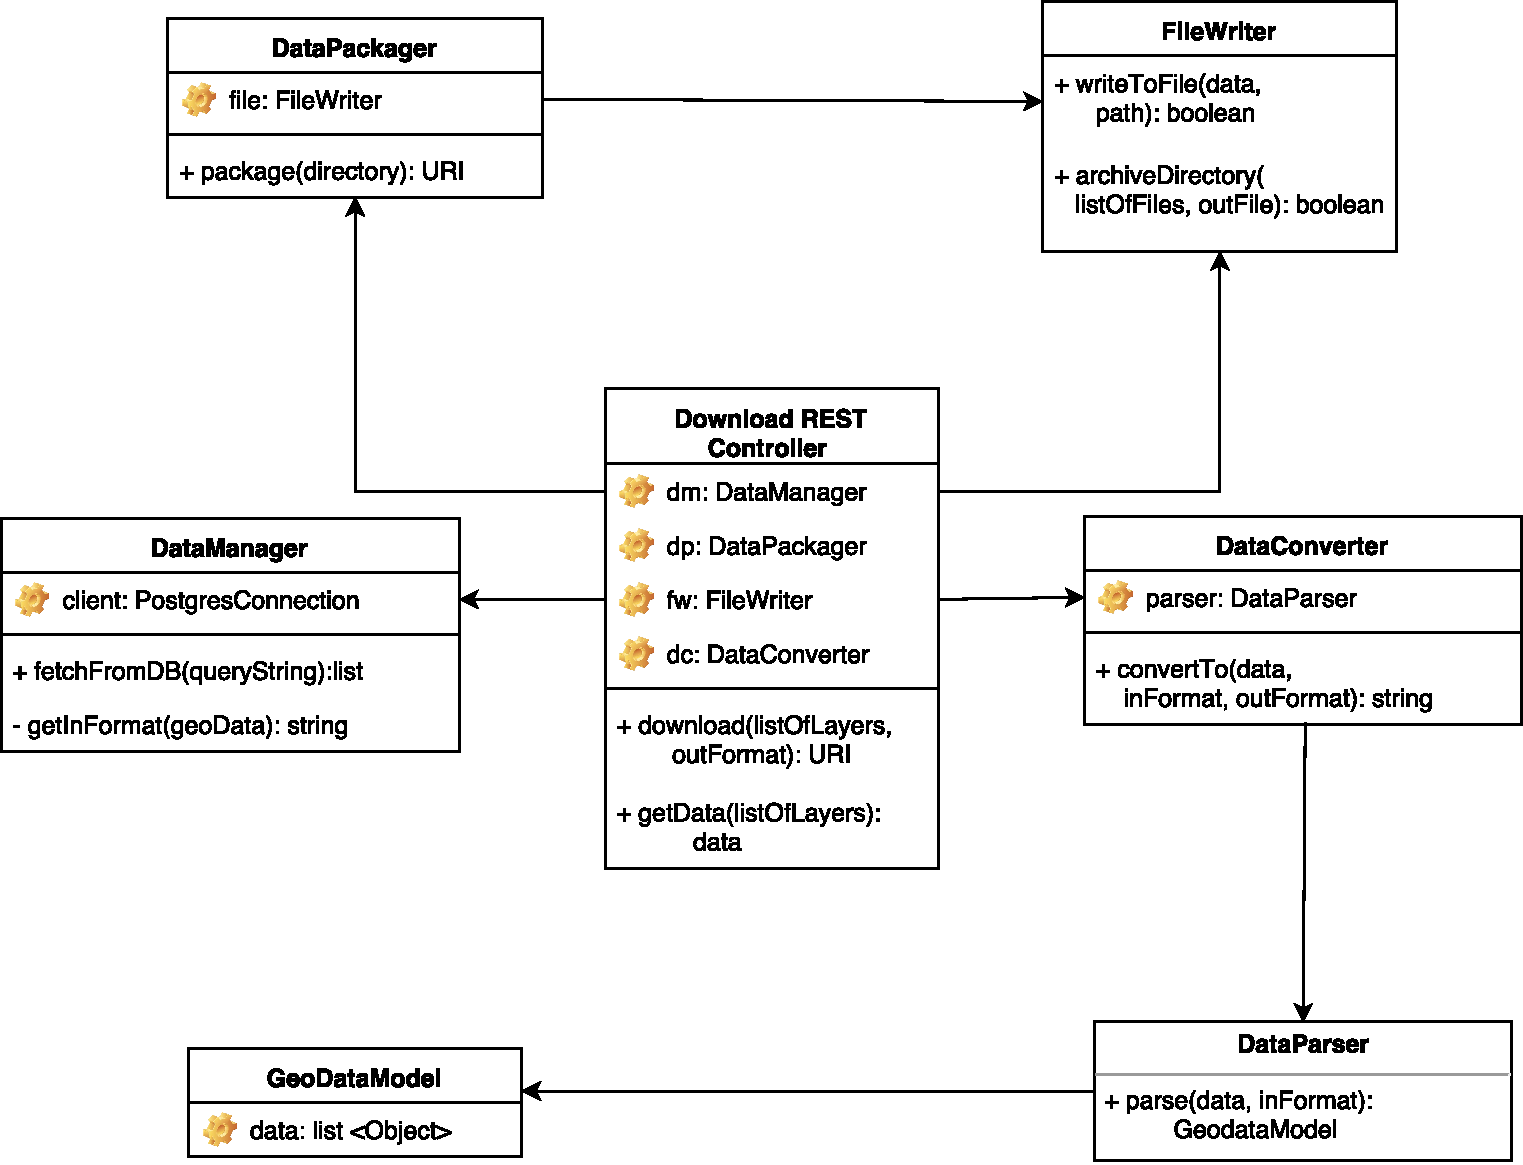
\includegraphics[width=\textwidth]{images/class_diagram.pdf}
		\end{center}
	\end{figure}
	
	\end{document}
	